% !TeX spellcheck = de_AT_frami
\documentclass[10pt,a4paper]{article}
\usepackage[utf8x]{inputenc}
\usepackage{ucs}
\usepackage{amsmath}
\usepackage{amsfonts}
\usepackage{amssymb}
\usepackage{bm}
\usepackage{graphicx}
\usepackage{txfonts}
\usepackage[dvipsnames]{xcolor}
\usepackage{geometry}
\usepackage{graphicx}
\usepackage{epstopdf}
\epstopdfsetup{update}
\geometry{margin= 2cm}
\usepackage{multirow}
\usepackage{cellspace}

\setlength\parindent{0pt}
\renewcommand*{\theenumi}{\thesection.\arabic{enumi}}
\renewcommand*{\theenumii}{\theenumi.\arabic{enumii}}

\begin{document}
	\pagenumbering{gobble}
	\title{VO Numerische Mathematik
		\\
		2017/18
		\\
		\flushbottom
		Theoriefragen }
	\maketitle
	
	\newpage
	\section{Zahldarstellung, Rundung und Fehler}
	\begin{enumerate}
		\item \textbf{Wie werden ganze Zahlen binär abgespeichert?}\\
			S. 2
			\begin{align*}
				b_{N-1}b_{N-2}\dots b_{1}b_{0} \cong b = \sum_{j=0}^{N-1}b_j2^j, \quad b_j\in\{0,1\}
			\end{align*}
			Beispiel: $23_{10}$
			\begin{align*}
					10101_2 &= 1\cdot2^4+0\cdot2^3+0\cdot2^2+1\cdot2^1+1\cdot2^0 \\
					      &= 16+0+0+2+1 = 19_{10}
			\end{align*} \vspace{-1cm}
			\begin{figure}[htbp]
				\centering
				\begin{minipage}{0.3\textwidth}
					\centering
					$$\begin{array}{rrrrrr}
					\multirow{2}{*}{:2} & 19 & 9 & 4 & 2 & 1 \\
					\cline{2-6}
					 \rule{0pt}{2.5ex} & 1 &  1 & 0 & 0 & 1
					\end{array}$$
				\end{minipage}\hspace{-0.5cm}
				\begin{minipage}{0.01\textwidth}
					\centering
					$\rightarrow$
				\end{minipage}\hspace{-0.7cm}
				\begin{minipage}{0.2\textwidth}
					\centering
					$10011_2$
				\end{minipage}
			\end{figure}
			
			
		\item \textbf{Wie werden Gleitpunktzahlen (doppelte Genauigkeit) binär abgespeichert?}\\
		S. 3
			\begin{align*}
				x &= (-1)^s \cdot m \cdot 2^e \\
				x &\cong s \;\;\; e_{11}e_{10}\dots e_0 \;\;\; (m_0).m_1m_2\dots m_{51}
			\end{align*}\vspace{-0.5cm}
			\begin{table}[htbp]
				\centering
				\begin{tabular}[htpb]{rll}
					s \; \dots \!\!\! & Vorzeichenbit &$\in \{0,1\}$\\
					m \; \dots \!\!\! & Mantisse & Normiert, $m_0\overset{!}{=}1$ wird weggelassen\\
					e \; \dots \!\!\! & Exponent & nach Abzug von b$\dots$Bias 
				\end{tabular}
			\end{table}
		
		\item \textbf{Wie werden Gleitpunktzahlen gerundet?} \\
		S. 6 \\
		Round to the nearest even.
		\item \textbf{Wie ist der relative Rundungsfehler definiert?} \\
		S. 6
		\begin{align*}
			\frac{|rd(x)-x|}{|x|}\leq \frac{2^{-M-1}\cdot2^e}{a\cdot 2^e}\underset{a\in[1,2)}{\leq}2^{-M-1}=:\texttt{eps}
		\end{align*}
		
		\item \textbf{Wie groß ist die relative Maschinengenauigkeit \texttt{eps} für doppelt genaue Gleitpunktzahlen?\\
					Wie kann man \texttt{eps} experimentell bestimmen?} \\
				
				
		\item \textbf{Was ist die relative/absolute Kondition eines Problems?} \\
		
		
		\item \textbf{Was bedeuten die Begriffe Konsistenz und Konsistenzordnung?} \\
		
		
		\item \textbf{Wodurch unterscheidet sich Konsistenz von Konvergenz?} \\
		
		
		\item \textbf{Was bedeutet der Begriff Stabilität?} \\
		S. 15\\
		Ein numerisches Verfahren $f$ heißt stabil, falls bei der numerischen Auswertung $f''(x)$ des Verfahrens Fehler wie Rundungsfehler, Abbruchfehler und Verfahrensfehler von Teilschritten nicht	übermäßig verstärkt werden im Vergleich zu dem durch die relative Kondition $\kappa_{rel}$ des Problems
		verursachten Fehler.
		
	\end{enumerate}
	\newpage
	% !TeX spellcheck = de_AT_frami
\section{Numerische Differentiation}
	\begin{enumerate}
		\item \textbf{Wie wird mit Hilfe der Vorwärtsdifferenz eine differenzierbare Funktion \(\mathbf{f}\) an der Stelle \(\mathbf{x}\) differenziert? Wie groß ist \(\mathbf{\text{h}_{\text{opt}}}\)?}
			\begin{align*}
				f(x)=\frac{f(x+h)-f(x)}{h}-\frac{h}{2}f''(\xi), \quad \text{h}_{\text{opt}}=\sqrt{\texttt{eps}}
			\end{align*}
		\item \textbf{Wie wird mit Hilfe der zentralen Differenz eine differenzierbare Funktion \(\mathbf{f}\) an der Stelle \(\mathbf{x}\) differenziert? Wie groß ist \(\mathbf{\text{h}_{\text{opt}}}\)}
			\begin{align*}
				f(x)=\frac{f(x+h)-f(x-x)}{2h}-\frac{h^2}{6}f'''(\xi), \quad \text{h}_{\text{opt}}=\sqrt[3]{\texttt{eps}}
			\end{align*}
		\item \textbf{Wie verhalten sich Verfahrensfehler und Rundungsfehler in Abhängigkeit von der Schrittweite \(\mathbf{h}\)? Machen Sie eine Skizze.}
			\begin{figure}[!htbp]
				\centering				
				\begin{minipage}{.4\textwidth}
					\centering
					\begin{align*}
						\abs{V(h)}&\leq C_\text{V} h \\
						\abs{R(h)}&\leq C_\text{R} \frac{\texttt{eps}}{h} \\
						\abs{\text{err}(h)}&\leq C_\text{V} h + C_\text{R} \frac{\texttt{eps}}{h}
					\end{align*}
				\end{minipage} %				
				\begin{minipage}{.5\textwidth}
					\centering
					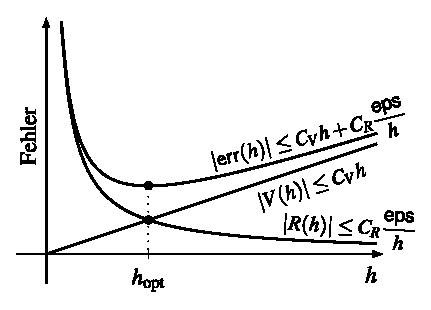
\includegraphics[width=0.8\linewidth]{Kap2_1}
				\end{minipage}
			\end{figure}			
		\item \textbf{Wie lässt sich mit Hilfe eines logarithmischen Plots das Verhalten von Verfahrensfehler und Rundungsfehler ablesen? Wie kann man die optimale Schrittweite \(\mathbf{h_{opt}}\) ablesen?}
			\begin{align*}
				\log \abs{\text{err}}=\log \left( C_\text{V} h + C_\text{R} \frac{\texttt{eps}}{h}\right) \approx 
					\begin{cases}
						\log\left(C_\text{R}\texttt{eps}h^{-q}\right) =-q\log h + \log C_\text{R}+\log\texttt{eps}  , & \text{links von }  \text{h}_\text{opt},\\
						\log\left(C_\text{V}\texttt{eps}h^p\right) =p\log h + \log C_\text{V} , & \text{rechts von }  \text{h}_\text{opt}.		\\	
					\end{cases}
			\end{align*}
			Somit erhält man zwei Geraden der Form \(y=kx+d\), wobei \(k=-\text{q}\) und \(k=\text{p}\) aus dem Plot abgelesen werden können.\\
			Die optimale Schrittweite kann man im Schnittpunkt der beiden Geraden erkennen. 
		\item \textbf{Wieso gilt bei der zentralen Differenz für den Verfahrensfehler \(\mathbf{V(h)=\mathscr{O}(h^2)}\) statt \(\mathbf{\mathscr{O}(h)}\)?}\\
			Für die zentrale Differenz werden die Taylorpolynome für \(f(x+h)\) und \(f(x-h)\) gemittelt. Dabei heben sich die Terme zweiter Ordnung, \(\frac{h^2}{2}f''(x)\), auf.
		\item \textbf{Wie wird die zweite Ableitung einer zweimal differenzierbaren Funktion an der Stelle \(\mathbf{x}\) berechnet? Wie groß ist \(\mathbf{h_{opt}}\)?}
			\begin{align*}
				f''(x)=\frac{f(x+h-2f(x)+f(x-h)}{h^2}-\frac{h^2}{12}f^{(4)}(\xi), \quad \text{h}_\text{opt}=\sqrt[\left( \text{q}+\text{p}\right) ]{\texttt{eps}}=\sqrt[4]{\texttt{eps}}
			\end{align*}
		\item \textbf{Wie lässt sich die optimale Schrittweite \(\mathbf{h_{opt}}\) aus dem Verfahrensfehler \(\mathbf{V(h)}\) und dem Rundungsfehler \(\mathbf{R(h)}\) bestimmen?}
			\begin{align*}
				\abs{\text{err}(h)}&\leq C_\text{V} h + C_\text{R} \frac{\texttt{eps}}{h}
			\end{align*}
			Der Fehler soll minimal sein und somit \(C_\text{V} h + C_\text{R} \frac{\texttt{eps}}{h}=\text{min}.\) Dies führt zu \(C_\text{V} h^2 + C_\text{R}\texttt{eps}=0\) und somit
			\begin{align*}
				\text{h}_\text{opt}=\sqrt{\texttt{eps}\frac{C_\text{V}}{C_\text{R}}}.
			\end{align*}			 
			Bei \(f(x)\approx f'(x) \approx f''(x)\) gilt \(C_\text{V} \approx C_\text{R}\) und somit
			\begin{align*}
				\text{h}_\text{opt}&=\sqrt{\text{eps}}
			\end{align*}
		\item \textbf{Wie berechnet man die Jacobimatrix einer vektorwertigen Funktion \(\mathbf{f:}{\rm I\!R}\mathbf{^n} \rightarrow {\rm I\!R}\mathbf{^m}\) durch numerisches Differenzieren?}\\
			Jacobimatrix: \(\mathbf{J(x)}=\mathbf{f'(x)})=\begin{bmatrix}
				\pd{f_1}{x_1} & \cdots & \pd{f_1}{x_n} \\
				\vdots &  & \vdots \\
				\pd{f_{m}}{x_1} & \cdots & \pd{f_m}{x_n}
			\end{bmatrix}\) \\\\
			Approximation der i-ten Spalte
			\begin{align*}
				\pd{\mathbf{f}}{x_i}(\mathbf{x})=
					\begin{bmatrix}
						\pd{f_1}{x_i}(\mathbf{x}) \\
						\vdots \\
						\pd{f_m}{x_i}(\mathbf{x})
					\end{bmatrix}
					\approx \frac{\mathbf{f}(x_1,\dots,x_{i-1},x_i+h,x_{i+1},\dots,x_n)-\mathbf{f(x)}}{h}
			\end{align*}
		\item \textbf{Wie berechnet man den Gradient einer skalaren Funktion \(\mathbf{f:}{\rm I\!R}\mathbf{^n} \rightarrow {\rm I\!R}\mathbf{^m}\) durch numerisches Differenzieren?}\\
	\end{enumerate}
	\newpage
	% !TeX spellcheck = de_AT_frami
\section{Interpolation}
	\begin{enumerate}
		\item \textbf{Wie werden die dividierten Differenzen berechnet?} \\
			Mit Hilfe eines Differenzenschema oder Differenzentableau. \\
			Allgemeines Differenzenschema für 5 Punkte
				\begin{align*}
				\begin{array}{cc|cccc}
					x_i & y_i &              \delta y_i              &                     \delta^2 y_i                     &                       \delta^3 y_i                       &                       \delta^4 y_i                       \\ \hline
					x_0 & y_0 &  \\
					    &     & \delta y_0 = \frac{y_1-y_0}{x_1-x_0} &  \\
					x_1 & y_1 &                                      & \delta^2 y_0 = \frac{\delta y_1-\delta y_0}{x_2-x_0} &  \\
					    &     & \delta y_1 = \frac{y_2-y_1}{x_2-x_1} &                                                      & \delta^3 y_0 = \frac{\delta^2 y_1-\delta^2 y_0}{x_3-x_0} &  \\
					x_2 & y_2 &                                      & \delta^2 y_1 = \frac{\delta y_2-\delta y_1}{x_3-x_1} &                                                          & \delta^4 y_0 = \frac{\delta^3 y_1-\delta^2 y_0}{x_4-x_0} \\
					    &     & \delta y_2 = \frac{y_3-y_2}{x_3-x_2} &                                                      & \delta^3 y_1 = \frac{\delta^2 y_2-\delta^2 y_1}{x_4-x_1} &  \\
					x_3 & y_3 &                                      & \delta^2 y_2 = \frac{\delta y_3-\delta y_2}{x_4-x_2} &  \\
					    &     & \delta y_3 = \frac{y_4-y_3}{x_4-x_3} &  \\
					x_4 & y_4 &
				\end{array}
			\end{align*}
		\item \textbf{Wie ist das Newtonsche Interpolationspolynom definiert?}
			\begin{align*}
				p(x)=y_0+(x-x_0)\delta y_0+(x-x_0)(x-x_1)\delta^2 y_0+\dots+(x-x_0)(x-x_1)\cdots(x-x_{n-1}) \delta^\text{n} y_0
			\end{align*}
		
		\item \textbf{Wie wird mit dem Hornerschema ein Polynom $\mathbf{p(x)=a_0+a_1x+\dots +a_nx^n}$ ausgewertet?} \\
			\begin{align*}
				p(x)=a_0+x(a_1+x(a_2+\cdots+x(a_{n-2}+x(a_{n-1}+x\,a_n))\cdots))
			\end{align*}
		\item \textbf{Wie wird mit dem Hornerschema ein Newtonsches Interpolationspolynom ausgewertet?}
			\begin{figure}[htbp]
				\centering
				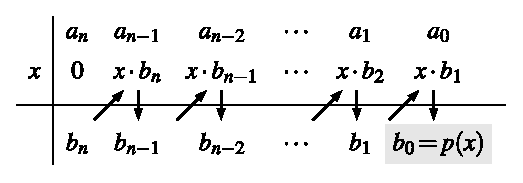
\includegraphics[width=0.45\linewidth]{Kap3_1}
			\end{figure}
		\item \textbf{Wie sind die Lagrange-Polynome definiert? Welche Eigenschaften haben sie?}
			\begin{align*}
				\ell_i(x)&=\frac{(x-x_0)(x-x_1)\cdots\reallywidehat{(x-x_i)}\cdots(x-x_n)}{(x_i-x_0)(x_i-x_1)\cdots\reallywidehat{(x_i-x_i)}\cdots(x_i-x_n)} \\
				\ell_i(x_j)&=\delta_{ij} =
					\begin{cases}
						1, & \text{falls } i=j,\\
						0, & \text{falls } i\neq j.
					\end{cases} \nonumber
			\end{align*}
			Wobei die überdachten Terme wegzulassen sind.
		\item \textbf{Wie wird mit Hilfe der Lagrange-Polynome das Langrangesche Interpolationspolynom berechnet?}
			\begin{align*}
				p(x)=\sum_{i=0}^{n}y_i\,\ell_i(x), \quad p(x_j)=y_j
			\end{align*}
		
		\pagebreak
		
		\item \textbf{Erklären Sie die Begriffe Datenfehler, Verstärkungsfaktor, Lebesgue-Funktion und Lebesgue-Konstante in Zusammenhang mit der Polynominterpolation. Was ist die Kondition der Polynominterpolation?} \\
			An einer Stützstelle \(x_j\) kann ein Datenfehler \(\varepsilon_j\) auftreten.
			Führt man diesen in ein Lagrange-Polynom ein erhält man
			\begin{align*}
				\overline{p}(x)=\sum_{i=0}^{j-1}\left( y_i\,\ell_i(x)\right) + (y_j+\varepsilon_j)+\sum_{i=j+1}^{n}\left( y_i\,\ell_i(x)\right).
			\end{align*}
			Der Fehler \(\varepsilon_i\) wird also um den Faktor \(|\ell_i|\) verstärkt.
			Wenn alle Knoten mit Fehlern verseht sind ergibt sich
			\begin{align*}
				\overline{p}(x)=p(x)+\sum_{i=0}^{n}\left( \varepsilon_i\,\ell_i \right) .
			\end{align*}
			Falls die einzelnen Fehler durch \(\varepsilon_i\le\text{M}\) beschränkt sind erhält man für den absoluten Fehler die Abschätzung
			\begin{align*}
				\underbrace{|\overline{p}(x)-p(x)|}_\text{abs. Fehler Output}\leq \text{M}\underbrace{\sum_{i=0}^{n}\overbrace{|\ell_i(x)|}^{\kappa_{\text{abs},i}(x)}}_{\kappa_\text{abs}(x)}
				= \text{M}\cdot\kappa_\text{abs}(x).
			\end{align*}
			Wobei \(\kappa_{\text{abs},i}=|\ell_i(x)|\) der Verstärkungsfaktor für den Datenfehler in der Stützstelle \(i\) und die Lebesgue-Funktion \(\kappa_\text{abs}=\lambda_n(x)=\sum_{i=0}^{n}|\ell_i(x)|\) die absolute Kondition für die Polynominterpolation ist. Die schlechteste Konditionszahl \(\lambda_n(x)\) im Intervall \([\text{min}_ix_i,\text{max}_ix_i]\) nennen wir Lebesgue-Konstante und erhalten sie durch
			\begin{align*}
				\underset{x\in[\text{min}_ix_i,\text{max}_ix_i]}{\text{max}} \lambda_n(x):=\Lambda_n.
			\end{align*}
		\item \textbf{Was besagt der Satz über den Fehler des Interpolationspolynoms? Wie ist der Verfahrensfehler definiert?} \\
			Gegeben seien \(n+1\) verschiedene Stützstellen \(x_i, i=0,\dots,n\), in einem Intervall \([a,b]\) und eine \(n+1\)-mal stetig differenzierbare Funktion \(f\in\mathscr{C}^{n+1}([a,b])\). Dann gilt für den Fehler \( f(x)-p(x) \) des Interpolationspolynoms folgende Aussage: \\
			Für alle \( x\in[a,b] \) gibt es ein \( \xi=\xi(x) \), das also von x abhängen kann, mit
			\begin{align*}
				\xi \in \left( \text{min}\{x_0,\dots,x_n,x \}, \text{max}\{x_0,\dots,x_n,x \} \right)
			\end{align*}
			sodass gilt:
			\begin{align*}
				f(x)-p(x)=(x-x_0)(x-x_1)\cdots(x-x_n)\frac{f^{(n+1)\left(\xi\right)}}{(n+1)!}.
			\end{align*}
			Somit ergibt sich für den Verfahrensfehler
			\begin{align*}
				\prod(x):=|(x-x_0)(x-x_1)\cdots(x-x_n)|.
			\end{align*}
		\item \textbf{Wie sind die Tschebyscheff-Polynome definiert? Welche Eigenschaften haben sie?} \\
			Die durch Abbildung \(T_n:[-1,1]\rightarrow[-1,1]\) mit
			\begin{align*}
				T_n(x)=\cos(n\arccos(x))
			\end{align*}
			definierten Polynome heißen Tschebyscheff-Polynome. Für sie gilt:
			\begin{enumerate}
				\item[(1)] \(T_n\) ist ein Polynom \(n\)-ten Grades in \(x=\cos\phi\).
				\item[(2)] Rekursionsformel für Tschebyscheff-Polynome:\\
						\(T_0(x)=1, T_1(x)=x\) und \(T_{n+1}(x)=2xT_n(x)-T_{n-1}(x),\,\, n=1,2,\dots\)
				\item[(3)] \(T_n(x)\leq1\) für \(x\in[-1,1] \).
				\item[(4)] \(T_n\) ist eine gerade oder ungerade Funktion, je nachdem, ob n gerade oder ungerade ist.
				\item[(5)] \(T_n\) besitzt ganzzahlige Koeffizienten. Der führende Koeffizient ist \(2^{n-1}\) für \(n\geq1\).
				\item[(6)] \(T_n\) nimmt für \(n\geq 1\) im Intervall \([-1,1]\) (n+1)-mal die Werte \(\pm1\) an, nämlich für \(x=\cos\frac{k\pi}{n},k=0,1,\dots,n\). Insbesondere gilt \(T_n(1)=1, T_n(-1)=(-1)^n\).
				\item[(7)] \(T_n\) hat \(n\) reelle Nullstellen in \([-1,1]\), nämlich die Tschebyscheff-Knoten
					\begin{align*}
						t_k^{(n)}=\cos\left( \frac{2k-1}{2n}\pi \right),\, k=1,\dots,n. 
					\end{align*}
			\end{enumerate}
		\item \textbf{Wie berechnet man die Knoten für die Tschebyscheff-Interpolationspolynome im Intervall \(\mathbf{[−1,1]}\) bzw. \(\mathbf{[a,b]}\)? Welche Vorteile hat die Verwendung von Tschebyscheff-Knoten im Vergleich zu äquidistanten Stützstellen.} \\
			\(T_n\) hat \(n\) reelle Nullstellen in \([-1,1]\), nämlich die Tschebyscheff-Knoten
			\begin{align*}
				t_k^{(n)}=\cos\left( \frac{2k-1}{2n}\pi \right),\, k=1,\dots,n. 
			\end{align*}
			Für \([a,b]\) wird die Transformation
			\begin{align*}
				[-1,1]\rightarrow[a,b], t\rightarrow x(t)=\frac{1}{2}(a+b)+\frac{1}{2}(b-a)t
			\end{align*}
			ausgeführt und man erhält die Tschebyscheff-Knoten in \([a,b]\)
			\begin{align*}
				x_k^{(n)}=\frac{a+b}{2}+\frac{b-a}{2}t_k^{(n)}.\quad t_k^{(n)} \text{ ist } k\text{-ter Tschebyscheff-Knoten in }[-1,1]
			\end{align*}
			Die Tschebyscheff-Interpolation ist wesentlich besser konditioniert.
			
		\item \textbf{Wie lässt sich das dividierte Differenzenschema und das Newtonsche Interpolationspolynom verallgemeinern, falls in den Stützstellen auch noch Ableitungen vorgegeben sind?} \\
			Durch Hermite-Interpolation. Idee: Interpolation durch die Punkte \((x_i,y_i),(x_i+h,y_i+hy_i'),i=0,\dots,n\), und Grenzübergang \(h\rightarrow0\). Führt zu Differenzenschema in dem Punkte doppelt angeschrieben und Werte für die man mit 0 dividieren müsste durch die gegebenen Ableitungen ersetzt werden.
			
		\item \textbf{Wie wird mit stückweise konstanten Funktionen interpoliert?} \\
			Das Intervall \([a,b]\) wird in \(n\) Intervalle unterteilt, wobei die Intervallsgrenzen genau zwischen den Knoten liegen. Die Treppenfunktion definiert sich aus den Intervallen \(I_i\) und den Stützstellen \(x_i\) zu
			\begin{align*}
				s(x)=\sum_{i=0}^{n}y_i\,\chi_i(x)
				\intertext{mit}
				\chi_i(x)=\begin{cases}
				1, & \text{falls } x\in I_i,\\
				0, &  sonst.
				\end{cases}
			\end{align*}
			\begin{figure}[htbp]
				\centering
				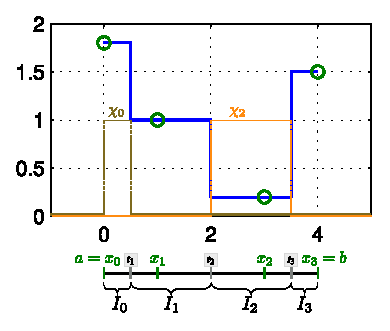
\includegraphics[width=0.4\linewidth]{Kap3_2}
			\end{figure}
		
		\pagebreak
		
		\item \textbf{Wie wird mit stetigen, stückweise linearen Funktionen interpoliert?} \\
			Wie oben, nur wird \(\chi_i\) ersetzt durch die Hutfunktion
			\begin{align*}
				\varphi_i=\begin{cases}
					\frac{x-x_{i-1}}{x_i-x_{i-1}}\,\,x\in[x_{i-1},x_i], & \text{falls } i=1,\dots,n \\
					\frac{x_{i+1}-x}{x_{i+1}-x_i}\,\,x\in[x_i,x_{i+1}], & \text{falls } i=0,\dots,n-1 \\
					0, \text{sonst}
				\end{cases}
			\end{align*}
			was analog zu konstanten Funktionen auf
			\begin{align*}
				s(x)=\sum_{i=0}^{n} y_i\,\varphi_i(x)
			\end{align*}
			führt.
			\begin{figure}[htbp]
				\centering
				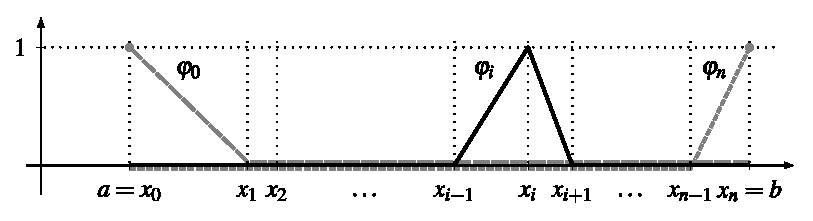
\includegraphics[width=0.6\linewidth]{Kap3_3}
			\end{figure}
				\begin{figure}[htbp]
				\centering
				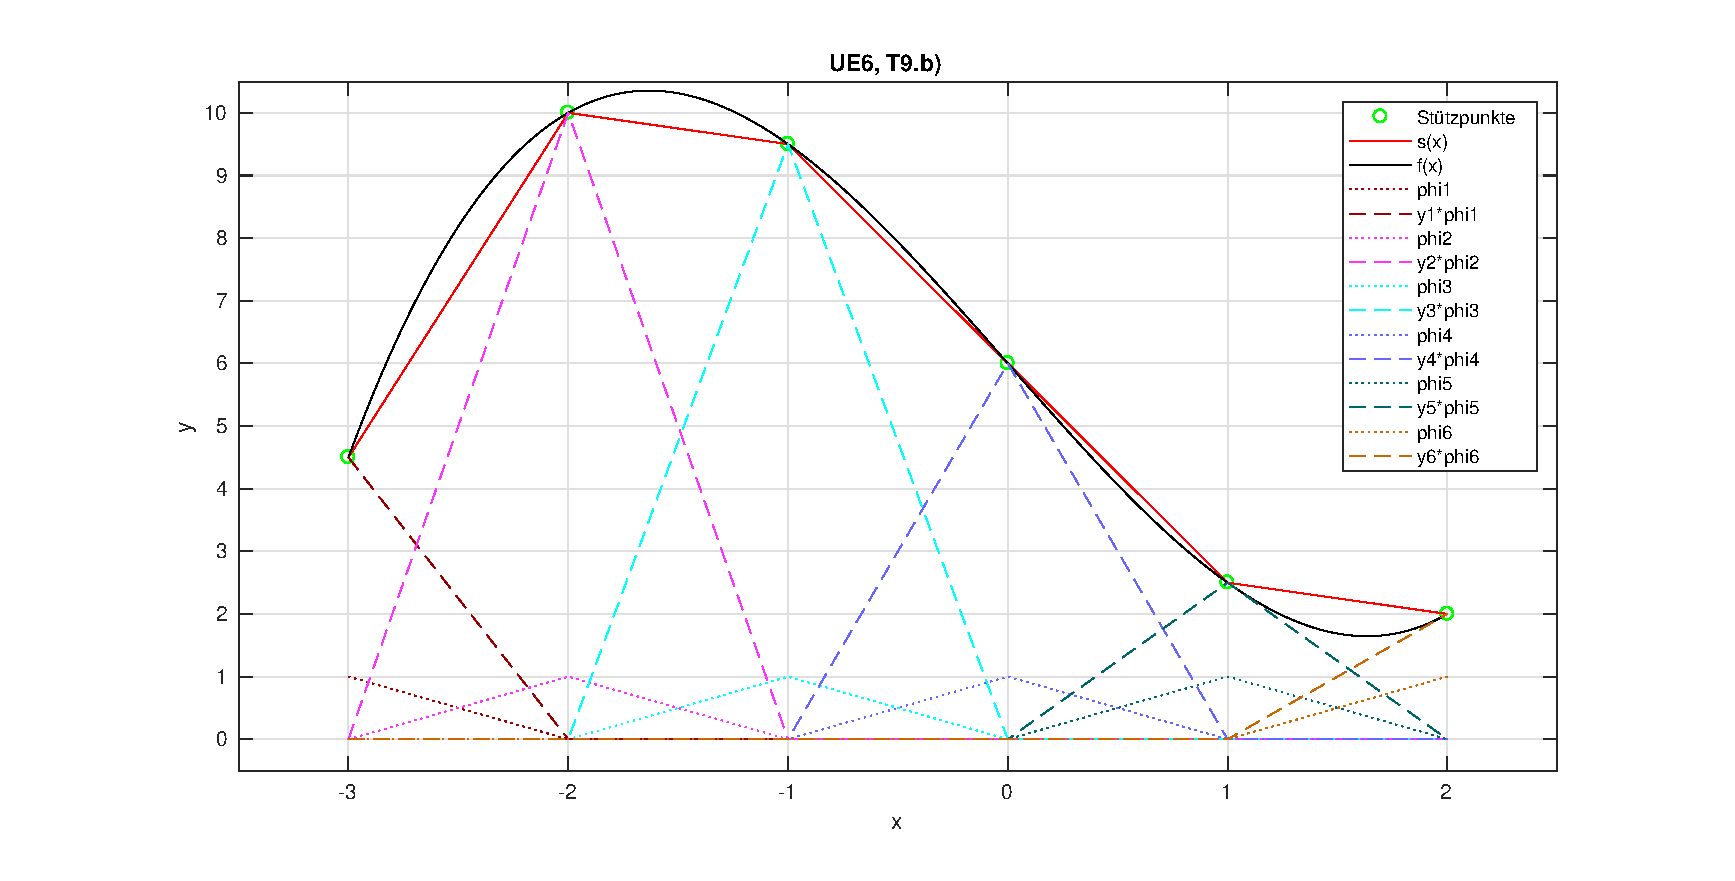
\includegraphics[width=1.0\textwidth]{T9b}
			\end{figure}
		
		\pagebreak
		
		
		\item \textbf{Was sind Hutfunktionen und welche Eigenschaften haben sie?} \\
			Stückweise lineare Funktionen
			\begin{align*}
				\varphi_i=\begin{cases}
							\frac{x-x_{i-1}}{x_i-x_{i-1}}\,\,x\in[x_{i-1},x_i], & \text{falls } i=1,\dots,n \\
							\frac{x_{i+1}-x}{x_{i+1}-x_i}\,\,x\in[x_i,x_{i+1}], & \text{falls } i=0,\dots,n-1 \\
							0, \text{sonst}
						\end{cases}
			\end{align*}
			für die gelten
			\begin{align*}
				\phi_i(x_k)=\delta_{ij}.
			\end{align*}
		\item \textbf{Was für Eigenschaften besitzen kubische Splines? Was für Typen von kubischen Splines gibt es?} \\
			Eigenschaften:
			\begin{itemize}
				\item \(s_i(x_i)=y_i,\,i=0,\dots,n\) (Interpolationsbedingung)
				\item \(s\in\mathscr{C}^2([a,b])\), d.h. zweimal stetig differenzierbar
				\item \(s_i:=\eval[0]{s}_{[x_i,x_{i+1}]} \in \mathbb{P}_3([x_i,x_{i+1}]),\,i=0,\dots,n-1.\)
			\end{itemize}
			Typen:
			\begin{itemize}
				\item Natürlicher Spline \\
					\(s''(x_0)=s''(x_n)=0\) \\
					Die Momente an beiden Enden sind 0.
				\item Eingespannter Spline (vollständiger Spline) \\
					\(s'(x_0)=y_0',\,s'(x_n)=y_n'\) \\
					Die beiden Enden sind eingespannt und die Steigungen vorgegeben.
				\item Periodischer Spline \\
					\( s(x_0)=s(x_n),\,s'(x_0)=s'(x_n),\,s''(x_0)=s''(x_n) \).
				\item Not a knot \\
					\(s'''\) ist stetig in \(x_1\) und \(x_{n-1}\) \\
					Auf den ersten und letzten beiden Intervallen wird ein durchgehendes Polynom dritten Grades verwendet.
			\end{itemize}
		\item \textbf{Wieso ist es besser durch viele Punkte einen kubischen Spline zu legen, statt ein Interpolationspolynom zu verwenden?} \\
			Polynome schaukeln sich am Rand auf und sind daher zur Interpolation ungeeignet, wenn man ein Polynom durch viele Punkte mit beliebigen, paarweise verschiedenen Abszissen legen will.
		
		\item \textbf{Wie wird auf einem rechteckigen Gitter zweidimensional interpoliert?} \\
			Analog zum eindimensionalen Fall benützen wir zwei Lagrange-Polynome
			\begin{align*}
				\ell_i(x)&=\frac{(x-x_0)(x-x_1)\cdots\reallywidehat{(x-x_i)}\cdots(x-x_n)}{(x_i-x_0)(x_i-x_1)\cdots\reallywidehat{(x_i-x_i)}\cdots(x_i-x_n)} \\
				L_j(y)&=\frac{(y-y_0)(y-y_1)\cdots\reallywidehat{(y-y_j)}\cdots(y-y_m)}{(y_j-y_0)(y_j-y_1)\cdots\reallywidehat{(y_j-y_j)}\cdots(y_j-y_m)}
			\end{align*}
			um auf das Interpolationspolynom
			\begin{align*}
				p(x,y)=\sum_{i=0}^{n}\sum_{j=0}^{m}z_{ij}\ell_i(x)L_j(y)
			\end{align*}
			zu kommen, wobei \( \ell_i(x)L_j(y) \) das zur Stützstelle \((x_i,y_j)\) gehörige Lagrange-Polynom ist. Wiederum gilt \linebreak \(l_i(x_i)L_j(y_j)=1\) und \(l_i(x_r)L_j(y_s)=0\) für alle anderen Punkte \((x_r,y_s)\neq(x_i,y_j)\) des Gitters. \\
			Nun kann man entweder primär von links nach rechts und dann von oben nach unten rechnen, oder umgekehrt, hier nur eine Art.\\
			\(p(x,y)\) wird umgeformt zu
			\begin{align*}
				p(x,y)=\sum_{j=0}^{m}\left(\sum_{i=0}^{n}z_{ij}l_i(x)\right)L_j(y)=\sum_{j=0}^{m}r_j(x)L_j(y).
			\end{align*}
			\(r_j(x)\) ist das eindeutige Interpolationspolynom vom Grad \(n\) durch die Punkte \( (x_0,y_i,z_{0j}),\dots,(x_n,y_j,z_{nj})\).
			
			
		\item \textbf{Wie wird die zweidimensionale, stetige, stückweise lineare Interpolierende auf einem rechteckigen Gitter bestimmt?} \\
			Wir betrachten nur ein Rechteck \([x_i,x_{i+1}]\times[y_j,y_{j+1}]\) in dem der Punkt \((x,y)\) liegt.
			\begin{align*}
				s(x,y)=z_{ij}\varphi_i(x)\Phi_j(y)+z_{i+1,i}\varphi_{i+1}(x)\Phi_j(x)+z_{i,j+1}\varphi_i(x)\Phi_{j+1}(y)+z_{i+1,j+1}\varphi_{i+1}(x)\Phi_{j+1}(y)
			\end{align*}
			Wobei \(\varphi_i\) und \(\Phi_j\) die Hutfunktionen in x- und y-Richtung sind.
		
	\end{enumerate}
	\newpage
	% !TeX spellcheck = de_AT_frami
\section{Numerische Integration}
	\begin{enumerate}
		\item \textbf{Was bedeutet \textit{Linearität} und \textit{Positivität} des Integrals?} \\
		Eigenschaften des Integrals und der numerischen Approximation.
		\begin{itemize}
			\item Linearität: \quad \(\int_{a}^{b}\left(\alpha f(x)+\beta g(x)\right)\dif{x} = \alpha \int_{a}^{b}f(x)\dif{x}+\beta\int_{a}^{b}g(x)\dif{x}\)
			\item Positivität: \quad \(f(x)\geq0\) für alle \(x\in[a,b]\Rightarrow\int_{a}^{b}f(x)\dif{x}\geq0.\)
		\end{itemize}
		
		\item \textbf{Erklären Sie den Begriff \textit{Quadraturformel}.} \\
			Eine Quadraturformel \(Q=(b_i,c_i)^s_{i=1}\) ist eine Näherungsformel
			\begin{align*}
				I(g)=\int_{0}^{1}g(t)\dif{t}\approx\sum_{i=1}^{s}b_ig(c_i)=:Q(g)
			\end{align*}
			zur numerischen Berechnung eines Integrals auf dem Intervall \([0,1]\). Die Zahlen \(b_1,\dots,b_s\) heißen Gewichte und \(c_1,\dots,c_s\) Knoten der Quadraturformel, \(s\) ist die Anzahl der Stufen.
			Für die Knoten wird
			\begin{align*}
				0\leq c_1<c_2<\cdots<c_s\leq1
			\end{align*}
			verlangt und für die Gewichte
			\begin{align*}
				b_1+b_2+\dots+b_s=1.
			\end{align*}
			Für ein beliebiges Intervall \([a,b]\) werden die Knoten von \([0,1]\) nach \([a,b]\) transformiert und es gilt
			\begin{align*}
				I(g)=\int_{a}^{b}g(t)\dif{t}\approx(b-a)\sum_{i=1}^{s}b_i\underbrace{f(a+c_i(b-a))}_{g(c_i)}=:Q(f,[ab]).
			\end{align*}
			\begin{figure}[htbp]
				\centering
				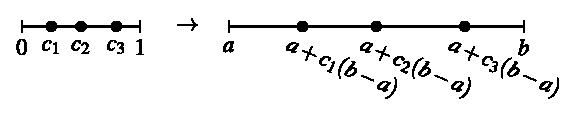
\includegraphics[width=0.4\linewidth]{kap4_1}
			\end{figure}
		
		
		\item \textbf{Nennen Sie einige einfache Quadraturformeln inklusive Knoten und Gewichte.}
			\begin{figure}[htbp]
				\centering
				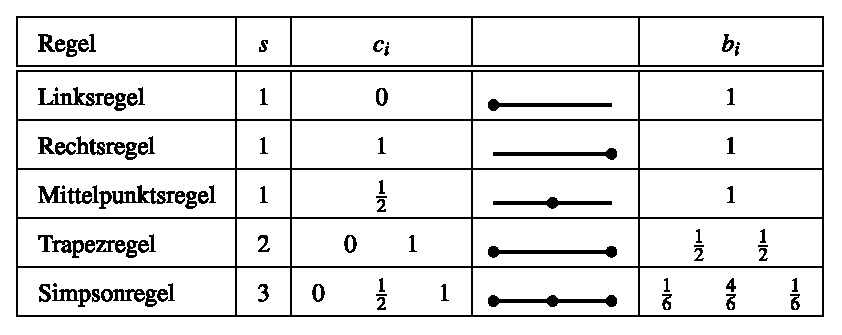
\includegraphics[width=0.6\linewidth]{kap4_2}
			\end{figure}
		
		\pagebreak
		
		\item \textbf{Erklären Sie den Begriff \textit{zusammengesetzte Quadraturformel}.} \\
			Ist der Abstand \(b-a\) sehr groß oder ändert sich der Integrand im Integrationsbereich \([a,b]\) rasch, zerlegt man \([a,b]\) in \(n\) Teilintervalle \([x_0,x_1],[x_1,x_2],\dots,[x_{n-1},x_n]\) mit \(a=x_0<x_1<x_2<\cdots<x_{n-1}<x_n=b\). Das Integral wird aufgespalten in eine Summe von \(n\) Teilintegralen über die einzelnen Teilintervalle:
			\begin{align*}
				\int_{a}^{b}f(x)\dif{x}=\int_{x_0}^{x_1}f(x)\dif{x}+\int_{x_1}^{x_2}f(x)\dif{x}+\cdots+\int_{x_{n-1}}^{x_n}f(x)\dif{x}
			\end{align*}
			Jedes dieser Teilintegrale \(\int_{x_{k-1}}^{x_k}f(x)\dif{x}\) wird mit einer Quadraturformel numerisch berechnet.\\
			Genauer Definiert mit der Definition aus 4.2: \\
			Es sei eine Quadraturformel \(Q=(b_i,c_i)^s_{i=1}\) und eine Unterteilung des Intervalls \([a,b]\) wie oben gegeben. Dann heißt eine Näherungsformel
			\begin{align*}
				\int_{a}^{b}f(x)\dif{x}\approx\sum_{k=1}^{n}Q(f,[x_{k-1}],x_k)=\sum_{k=1}^{n}h_k\sum_{i=1}^{s}b_if(x_{k-1}+c_ih_k)=:S_Q(f,x_0,\dots,x_n)
			\end{align*}
			mit \(h_k=x_k-x_{k-1}\) zusammengesetzte Quadraturformel oder Summe von Quadraturformeln. Für eine äquidistante Unterteilung von \([a,b]\) in \(n\) Teilintervalle, also
			\begin{align*}
				x_k=a+kh, \quad h=\frac{b-a}{n}, \quad k=0,\dots,n,
			\end{align*}
			haben wir folgende Näherungsformel
			\begin{align*}
				\int_{a}^{b}f(x)\dif{x}\approx h\sum_{k=1}^{n}\sum_{i=1}^{s}b_if(x_{k-1}+c_ih)=:S_Q(f,h,[a,b])=S_Q(f,h).
			\end{align*}
		
		\item \textbf{Wie erhält man Quadraturformeln mit Hilfe von Polynominterpolation?} \\
			
		
		\item \textbf{Erklären Sie den Begriff \textit{Ordnung} einer Quadraturformel. Wie bestimmt man die Ordnung?} \\
		
		\item \textbf{Was sind \textit{Bedingungsgleichungen}?} \\
		
		\item \textbf{Erklären Sie die Begriffe \textit{Fehler einer Quadraturformel} und \textit{Fehlerkonstante}.} \\
		
		\item \textbf{Was für Abschätzungen gelten für den Fehler einer Quadraturformel bzw. einer zusammengesetzten Quadraturformel? Was muss der Integrand $f$ dabei erfüllen?} \\
		
		\item \textbf{Was sind \textit{symmetrische Quadraturformeln} und welche Eigenschaft besitzen sie?} \\
		
		\item \textbf{Was ist eine Gaußsche Quadraturformel? Welche Ordnung besitzen sie?} \\
		
		\item \textbf{Wie groß kann die Ordnung einer Quadraturformel maximal sein?} \\
		
		\item \textbf{Was gilt für die Gewichte einer Gaußschen Quadraturformel?} \\
		
		\item \textbf{Wie funktioniert eine Schrittweitensteuerung? Erklären Sie die Begriffe \textit{Fehlerkriterium} und \textit{Fehlerschätzer}.} \\
		
		\item \textbf{Erklären Sie den Begriff \textit{Richardson-Extrapolation}. Wie berechnet man est und $\mathbf{Q_extr}$.} \\
		
		\item \textbf{Was passiert bei Integranden mit Singularitäten oder Singularitäten in den Ableitungen?} \\
		
		\item \textbf{Wie werden Doppelintegrale auf Rechtecken numerisch berechnet?} \\
		
		\item \textbf{Wie werden Doppelintegrale auf Dreiecken numerisch berechnet? Wie überprüft man die Ordnung einer Quadraturformel für Dreiecke?} \\
		
		\item \textbf{Was sind \textit{baryzentrische Koordinaten}?} \\
		
	\end{enumerate}
\end{document}